\documentclass[12pt]{article}
\usepackage[utf8]{inputenc}
\usepackage[T1]{fontenc}
\usepackage{amsmath, amssymb, amsfonts, amsthm, minted}
\usepackage[top=1in, bottom=1in, left=1in, right=1in]{geometry}
\usepackage{graphicx, caption, subcaption}
\usepackage[numbers]{natbib}
\usepackage{tikz}
\usetikzlibrary{positioning,calc,shapes,arrows}
% Define block styles XXX
\tikzstyle{block} = [rectangle, draw,
    text width=8em, text centered, minimum height=5em]
\tikzstyle{line} = [draw, -latex',line width=1mm]

\bibliographystyle{plainnat}

\providecommand{\abs}[1]{\left\lvert#1\right\rvert}
\providecommand{\norm}[1]{\left\lVert#1\right\rVert}

\title{CS 240H Project Report: \\ Linear Least Squares Modeling in Haskell}
\author{Tri Dao \\ \texttt{trid@stanford.edu}}
\date{March 18, 2016}
\begin{document}

\maketitle

\section{Introduction}

Least squares are optimization problems that minimize the norm square
of an affine expression, subject to linear constraints on the variables.
They have the general form
\begin{equation}
  \begin{array}{ll}
    \mbox{minimize} & \|Ax-b\|^2 \\
    \mbox{subject to} & Cx = d
  \end{array}
  \label{eq:std_form}
\end{equation}
where $x \in \mathbb{R}^{n}$ is a variable, $A \in \mathbb{R}^{m \times n}$ and
$C \in \mathbb{R}^{p \times n}$ are matrices, and $b \in \mathbb{R}^m$ and
$d \in \mathbb{R}^p$ are vectors.

These problems are routinely solved in the context of statistical estimation,
machine learning, and engineering design.
For example, linear regression, an approach for modeling the relationship
between a scalar dependent variable $y$ and one or more explanatory variables
$X$, involves solving the problem minimize $\norm{X \beta - y}^2$ to find
$\beta$, where $X$ is a given data matrix, $y$ is a given vector, and $\beta$ is
the \emph{parameter vector}.

In general, there can be many variables, the objective can contain many
quadratic terms, and there can be multiple linear constraints.
Typically one has to rewrite the problem in the standard
form~\eqref{eq:std_form} and then use a general solver implemented by many
numerical linear algebra packages.
However, this is a tedious and error-prone process, especially for problems with
many variables or several linear constraints.

We aim to develop a modeling language embedded in Haskell to solve these
linearly constraints least squares problems.
This modeling language (in Haskell) will allow user to specify the problem in a
natural way that mirrors standard mathematical notation without being
constrained by the standard form.

\section{Background}

\subsection{Solution to the least squares problem}

The (unconstrained) \emph{least squares problem} has the standard form
\begin{equation*}
  \begin{array}{ll}
    \mbox{minimize} & \|Ax-b\|^2,
  \end{array}
\end{equation*}
where $x \in \mathbb{R}^n$ is a variable, $A \in \mathbb{R}^{m \times n}$ is a
matrix, and $b \in \mathbb{R}^m$ is a vector.
Assuming that $A$ is full rank, the least squares problem has the close-form
solution
\begin{equation*}
  \hat x = (A^T A)^{-1} A^T b.
\end{equation*}

A slight generalization is the (linearly) \emph{constrained least squares problem}:
\begin{equation*}
  \begin{array}{ll}
    \mbox{minimize} & \|Ax-b\|^2 \\
    \mbox{subject to} & Cx = d
  \end{array}
\end{equation*}
where $x \in \mathbb{R}^{n}$ is a variable, $A \in \mathbb{R}^{m \times n}$ and
$C \in \mathbb{R}^{p \times n}$ are matrices, and $b \in \mathbb{R}^m$ and
$d \in \mathbb{R}^p$ are vectors. The solution of this constrained problem is
\begin{equation*}
  \left[\begin{array}{c} \hat x \\ z \end{array}\right] =
  \left[\begin{array}{cc} 2A^TA & C^T \\ C & 0 \end{array}\right]^{-1}
  \left[\begin{array}{c} 2A^Tb \\ d \end{array}\right],
\end{equation*}
where $z$ is the dual variable to the equality constraint.
We assume that the matrix above is invertible.
This occurs when the matrix $C$ has independent rows, and the matrix
$\begin{bmatrix} A \\ C \end{bmatrix}$ has independent columns.

\subsection{Numerical linear algebra in Haskell}

We use the package \verb|hmatrix|~\cite{ruiz2015hmatrix-0.17.0.1} to handle
vectors and matrices.
This is a purely functional interface to linear algebra and other numerical
algorithms, internally implemented using LAPACK, BLAS, and GSL.

The types provided (\verb|Matrix| and \verb|Vector|) are dense, immutable and
strict in all elements (unboxed).
We will only use the double precision real versions of these types, i.e.
\verb|Matrix R| and \verb|Vector R| (\verb|R=Double|).
The matrix product is \verb|(<>)|, the matrix-vector product is \verb|(#>)|, the
dot product is \verb|(<.>)|, and the (conjugate) transpose is \verb|tr|.

\section{Modeling}

The key data type is a linear expression \verb|LinExpr|, which contains
variables and constants that are combined using linear mathematical functions
(addition, scaling, matrix-vector multiplication, etc.).
A linear constraint (type \verb|LinContr|) can be form as
\verb|LinExpr :==: LinExpr|.
A quadratic expression \verb|QuadExpr| can be formed by taking square norm
(\verb|SumSquares|) of linear expressions, or sum of many such square norms.

The package provides a function \verb|minimize| to solve a least squares problem:
\begin{minted}{haskell}
minimize :: QuadExpr -> [LinContr] -> M.Map VarName (Vector R)
\end{minted}
The function takes a quadratic expression as objective, a list of linear
constraints, and returns a map from variable names (type alias for
\verb|String|) to variable values.

For example, the classic problem of find the least norm solution to an
under-determined system can be easily setup and solved with the following code:
\inputminted{haskell}{app/example_least_norm.hs}

\section{Implementation}

Given a problem with a quadratic expression as objective and a list of linear
constraints, the system will analyze the abstract syntax tree to transform it to
the standard form in~\eqref{eq:std_form}, and then solve it using linear
algebra subroutines.

The three steps of solving a least squares problem is given in Figure~\ref{fig:steps}.
\begin{figure}[!ht]
  \centering
  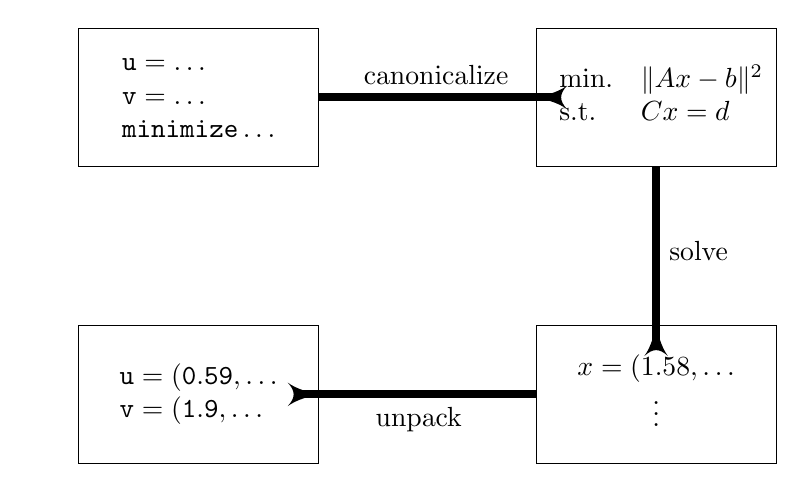
\begin{tikzpicture}[auto]
      % Place nodes
      \node (left_up) {};
      % \node [below=1cm of left_up] (left_down) {};
      \node [block,right=4mm of left_up] (code) {$\begin{array}{l}
      \tt{u = \ldots} \\
      \tt{v = \ldots} \\
      \tt{minimize \ldots}
      \end{array}$};
      \node [block, right =2.75cm of code] (cone) {$\begin{array}{ll}
  \mbox{min.}  &\|Ax-b\|^2 \\
  \mbox{s.t.} &Cx = d
  \end{array}$};
      \node [block, below =2cm of cone] (sltn) {$\begin{array}{c}
  x = (1.58,\ldots \\
  \vdots
  \end{array}$};
      \node [block, left =2.75cm of sltn] (unpack) {$\begin{array}{l}
      \tt{u = (0.59,\ldots}\\
      \tt{v = (1.9,\ldots}
      \end{array}$};
  \path [line] (code) -- node {canonicalize} ++(4.5,0) -- (cone);
  \path [line] (cone) -- node {solve} ++(0,-3.0) -- (sltn);
  \path [line] (sltn) -- node {unpack} ++(-4.5,0) -- (unpack);
  \end{tikzpicture}
  \caption{Three steps of solving a least squares problem.}
  \label{fig:steps}
\end{figure}

In the canonicalization step, we stack all the variables in the problem as one
big variable, and then stack the linear constraints.
For example, given constraints $Cu + Dv = w$ and $Eu = z$, we produce the equivalent
constraint
\begin{equation*}
  \begin{bmatrix} C & D \\ E & 0 \end{bmatrix} \begin{bmatrix} u \\
    v \end{bmatrix} = \begin{bmatrix} w \\ z \end{bmatrix}.
\end{equation*}
Since the objective is a sum of square norms, we convert this sum to a single
equivalent square norm.
For example, if the objective is $\norm{Au - b}^2 + 2\norm{v}^2$, the equivalent
square norm is
\begin{equation*}
  \norm{\begin{bmatrix} A & 0 \\ 0 & \sqrt{2}I \end{bmatrix} \begin{bmatrix} u
      \\ v \end{bmatrix} - \begin{bmatrix} b \\ 0 \end{bmatrix} }^2,
\end{equation*}
where $I$ is the identity matrix.
We then form a new variable $x = \begin{bmatrix} u \\ v \end{bmatrix}$ and thus
both the objective and the constraints are transformed to standard form.

In the solve step, we simply call the least squares solver provided by
\verb|hmatrix|. The unpacking step takes the resulting vector and assign the
values to the original variables.

\section{Example}

We consider an example of least squares modeling in image de-blurring. Suppose
that $x$ is an image, $A$ is a blurring operator, and $y = Ax + v$ is a blurred,
noisy image that we are given. We choose $x$ to minimize
\begin{equation*}
 \|Ax -  y\|^2 + \lambda (\|D_\mathrm v x\|^2 + \|D_\mathrm h x\|^2),
\end{equation*}
where $D_\mathrm v$, $D_\mathrm h$ are vertical and horizontal differencing
operations and the scalar parameter $\lambda$ controls smoothing of de-blurred
image. The problem can be expressed in this natural form:
\begin{minted}{haskell}
minimize (SumSquares (a*x-b) + lambda * (SumSquares (dv*x) + SumSquares (dh*x))) []
\end{minted}

We show the burred, noisy image and the recovered image with $\lambda = 0.007$
in Figure~\ref{fig:images}.
\begin{figure}[!ht]
  \centering
  \begin{subfigure}{0.49\textwidth}
    \centering
    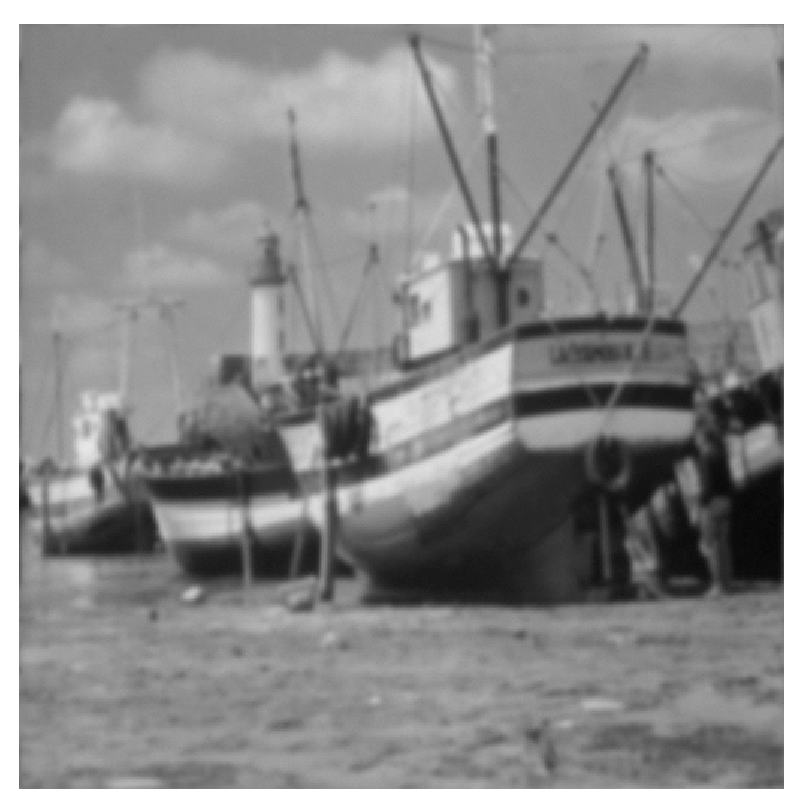
\includegraphics[width=0.8\textwidth]{figures/boat_blurred}
    \caption{Blurred, noisy image}
  \end{subfigure}
  \begin{subfigure}{0.49\textwidth}
    \centering
    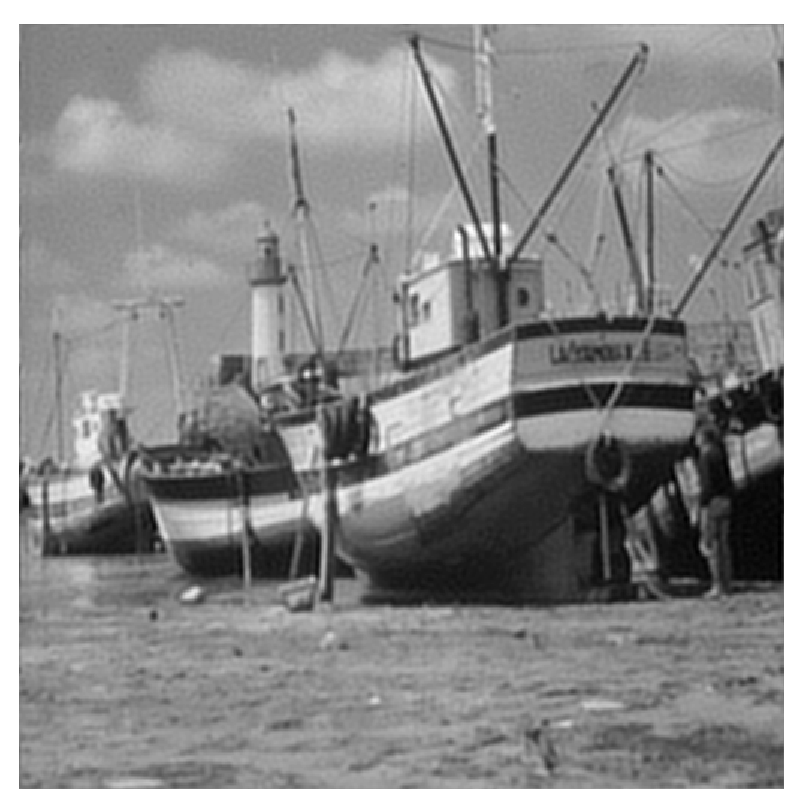
\includegraphics[width=0.8\textwidth]{figures/boat_deblurred}
    \caption{Recovered image}
  \end{subfigure}
  \caption{Blurred, noisy image and regularized inversion with $\lambda = 0.007$.}
  \label{fig:images}
\end{figure}

\section{Conclusion}

We have designed and implemented a modeling language embedded in Haskell for
linearly constrained least squares problem.
There are still some work to be done to add more linear operators (vector
indexing, convolution, Fourier transform, vector and matrix stacking, element
wise multiplication, etc.).
Moreover, the package only supports dense matrices due to lack of sparse matrix
support in Haskell.

Overall, this modeling language will allow users to express their problems in a
natural form while the system takes care of transforming it to the standard
form.
This might lead to faster prototyping and data analysis in statistical
estimation, machine learning, and engineering design.

\section*{Acknowledgment}

We thank Professor Stephen Boyd for introducing us to many examples of least
squares modeling in control, statistical estimation, and engineering design.
We also thank David Zeng whose Julia package \verb|LinearLeastSquares|
\cite{zeng2014linearleastsquares} inspired this project.

\bibliography{report}

\end{document}
%%% Local Variables:
%%% mode: latex
%%% TeX-master: t
%%% End:
